% Artículo IEEE del proyecto SAPDT (Hito 2, Calidad de Software).
% Compilar en Overleaf o con: pdflatex articulo_sapdt.tex (dos veces).
\documentclass[conference]{IEEEtran}
\usepackage[utf8]{inputenc}
\usepackage[T1]{fontenc}
\usepackage[spanish]{babel}
\usepackage{graphicx}
\usepackage{url}
\usepackage{booktabs}
\graphicspath{{../capturas/}{../diagramas/}}

\begin{document}

\title{SAPDT: Sistema de Análisis y Proyección de Demanda Turística Regional con Datos Abiertos y Aseguramiento de la Calidad de Datos en la Nube}

\author{
\IEEEauthorblockN{Nicolle Andrea Lozano Vega, Leonardo Raphael Pachari Gomez, Piero Fabricio Poblete Andía,\\
Katherine Naomi Saico Ccahuana y Davis Yovanny Arapa Chua}
\IEEEauthorblockA{Escuela de Ingeniería de Software, Universidad La Salle\\
Arequipa, Perú\\
\{nlozanov, lpacharig, ppobletea, ksaicoc, daparac\}@ulasalle.edu.pe}
}

\maketitle

\begin{abstract}
La planificación turística regional en el Perú suele apoyarse en la intuición porque los datos abiertos disponibles no son uniformes: cambian de esquema entre años, mezclan formatos decimales y contienen filas dañadas. Este artículo presenta SAPDT, una aplicación web desplegada en Google Cloud Run que consolida once años de indicadores de ocupabilidad hotelera del MINCETUR (enero de 2015 a junio de 2025) y el directorio de 5\,091 establecimientos de hospedaje clasificados, para ofrecer un dashboard regional, la clasificación de temporadas, la proyección de arribos a 3 y 6 meses, comparativos entre regiones y exportación a CSV y PDF. El desarrollo siguió un modelo incremental con Scrum adaptado y un catálogo de ocho requisitos funcionales y seis no funcionales basados en ISO/IEC 25010. La carga procesó 66\,981 filas sin rechazos, dejó 243 filas marcadas como observadas, 15 de ellas reparadas de forma verificable; el cruce produjo 25 regiones por 126 meses sin huecos. Sobre un periodo de validación de 12 meses, el modelo estacional ingenuo obtuvo un MAPE medio de 10,7\,\%, frente a 11,8\,\% del suavizado exponencial y 12,7\,\% del promedio móvil. Los resultados muestran que tratar la calidad de los datos como requisito verificable permite construir reportes confiables con una infraestructura de costo prácticamente nulo.
\end{abstract}

\renewcommand{\abstractname}{Abstract}
\begin{abstract}
Regional tourism planning in Peru often relies on intuition because open data is not uniform across years. This paper presents SAPDT, a web application deployed on Google Cloud Run that consolidates eleven years of MINCETUR hotel occupancy indicators and a directory of 5,091 classified lodging establishments to provide a regional dashboard, season classification, 3- and 6-month arrival forecasts, inter-regional comparisons and CSV/PDF export. Development followed an incremental, adapted Scrum process with eight functional and six ISO/IEC 25010-based non-functional requirements. The ingestion loaded 66,981 rows with no rejections, flagged 243 rows, 15 of them verifiably repaired; a seasonal naïve model reached a mean MAPE of 10.7\,\% on a 12-month hold-out.
\end{abstract}

\begin{IEEEkeywords}
calidad de software, calidad de datos, pruebas de software, ISO/IEC 42001, datos abiertos, ISO/IEC 25010, demanda turística, proyección, Cloud Run, Scrum.
\end{IEEEkeywords}

\section{Introducción}
El turismo es una actividad clave para regiones como Arequipa y Cusco, y decisiones como contratar personal, invertir en habitaciones o lanzar promociones dependen de saber cuándo llegan los visitantes y cuántos. La Plataforma Nacional de Datos Abiertos del Perú publica los indicadores mensuales de ocupabilidad de los hospedajes y el directorio de establecimientos clasificados del MINCETUR \cite{pnda,mincetur}, pero usarlos directamente es riesgoso: el esquema de los archivos cambia entre años, el separador decimal varía y algunas filas llegan partidas. Un reporte construido sin controlar estos problemas puede verse correcto y, aun así, mostrar cifras equivocadas.

El objetivo del trabajo fue desarrollar un producto de software que responda tres preguntas de planificación (cuántos turistas llegarán, cuándo es temporada alta y cuánta oferta de hospedaje existe) conservando durante todo el desarrollo un proceso de calidad de software. La contribución principal es tratar la calidad de los datos como un requisito verificable: cada fila rechazada, observada o reparada queda registrada con su motivo y cada regla de dominio tiene una prueba automática.

El resto del artículo se organiza así: la Sección~\ref{sec:relacionados} revisa trabajos relacionados; la Sección~\ref{sec:metodologia} describe el proceso y los estándares; la Sección~\ref{sec:requisitos} presenta los requisitos; la Sección~\ref{sec:arquitectura}, la arquitectura en la nube; la Sección~\ref{sec:resultados}, los resultados y pruebas; la Sección~\ref{sec:42001}, la relación con la ISO/IEC 42001; y la Sección~\ref{sec:conclusiones}, las conclusiones.

\section{Trabajos relacionados}\label{sec:relacionados}
La predicción de la demanda turística es un campo con amplia literatura. Song y Li \cite{song2008} revisan más de cien estudios y concluyen que ningún modelo supera a los demás en todos los contextos, y que los métodos simples de series de tiempo suelen ser competitivos frente a modelos más complejos. Hyndman y Athanasopoulos \cite{hyndman2021} recomiendan comparar todo modelo contra referencias simples, como el método estacional ingenuo, y Gardner \cite{gardner1985} sistematiza el suavizado exponencial, uno de los dos modelos que ofrece SAPDT. Para medir el error se usan MAE y MAPE, cuyas ventajas y límites discuten Hyndman y Koehler \cite{hyndman2006}.

En calidad de datos, Wang y Strong \cite{wang1996} muestran que la calidad depende del uso que el consumidor hace del dato e incluye dimensiones como exactitud, completitud y consistencia. La norma ISO/IEC 25012 \cite{iso25012} formaliza estas dimensiones, y la ISO/IEC 25010 \cite{iso25010} define el modelo de calidad del producto de software que el curso adopta para los requisitos no funcionales. En el plano normativo, la familia ISO/IEC 25000 (SQuaRE) reemplazó a la ISO/IEC 9126 y a la ISO/IEC 14598 como marco para especificar y evaluar la calidad del producto; la ISO/IEC/IEEE 12207 \cite{iso12207} define los procesos del ciclo de vida del software; IEEE 730 \cite{ieee730} establece el plan de aseguramiento de la calidad (SQA), e IEEE 829 \cite{ieee829} la documentación de pruebas. En pruebas, el programa ISTQB \cite{istqb2023} organiza los niveles (componente, integración, sistema y aceptación) y las técnicas de diseño de casos de caja negra, caja blanca y estáticas. Para sistemas que usan inteligencia artificial, la ISO/IEC 42001:2023 \cite{iso42001} es la primera norma de sistema de gestión de IA. Especifica requisitos para establecer, implementar, mantener y mejorar continuamente ese sistema de gestión en cualquier organización que provea o use productos basados en IA. Sigue la estructura armonizada de las normas de gestión (cláusulas 4 a 10: contexto, liderazgo, planificación, apoyo, operación, evaluación del desempeño y mejora) e incluye la evaluación de riesgos y de impacto de los sistemas de IA. Su Anexo A propone controles sobre, entre otros temas, la evaluación de impactos (A.5), el ciclo de vida del sistema de IA (A.6) y los datos para sistemas de IA (A.7), con controles de calidad, procedencia y preparación de los datos \cite{iso42001,modulos42001}. SAPDT combina ambas líneas: modelos de proyección simples y evaluados, sobre datos cuya calidad se controla y se informa.

\section{Metodología}\label{sec:metodologia}
\subsection{Modelo de proceso}
Se eligió un modelo incremental con Scrum adaptado \cite{scrum2020,sommerville2011} por tres razones: la calidad real de los datos solo se conoce al explorarlos, lo que exige un sprint inicial de exploración; el semestre tiene dos hitos de revisión, que piden entregas incrementales verificables; y el modelo permite ajustar el catálogo tras cada incremento sin rehacer un plan en cascada. La Tabla~\ref{tab:sprints} resume los sprints.

\begin{table}[t]
\caption{Sprints del proyecto}\label{tab:sprints}
\centering
\begin{tabular}{@{}lll@{}}
\toprule
Sprint & Contenido & Hito \\
\midrule
0 Exploración & Perfilado, catálogo, cronograma, diagramas & 1 \\
1 Datos & RF-01 ingesta y RF-02 cruce & 1 \\
2 Análisis y producto & RF-03 a RF-08, pruebas, despliegue & 2 \\
\bottomrule
\end{tabular}
\end{table}

El cronograma se planificó en 11 semanas desde el 1 de septiembre de 2026 con un diagrama de Gantt. Las semanas 1 a 4 pasaron sin avance formal; el retraso se recuperó paralelizando RF-01 y RF-02 en lugar de extender el calendario. El equipo se organizó en cuatro frentes: datos e ingesta (P.~Poblete y D.~Arapa), análisis y proyección (K.~Saico), producto y reportes (L.~Pachari) y calidad y documentación (N.~Lozano). El frente de datos llevó dos personas por concentrar el mayor riesgo.

\subsection{Gestión de la calidad}
Los requisitos se especificaron siguiendo las recomendaciones de IEEE 830 \cite{ieee830}, cada uno con criterios de aceptación verificables, y los no funcionales se derivaron de las características de ISO/IEC 25010 \cite{iso25010}. Se mantuvo una matriz de trazabilidad requisito, caso de uso, componente y prueba. La configuración se gestionó con Git y GitHub, y los diagramas (casos de uso, componentes y flujo de datos) se elaboraron con la herramienta CASE PlantUML, con sus fuentes en el repositorio.

\subsection{Verificación, validación y estrategia de pruebas}
Siguiendo a Pressman y Maxim \cite{pressman2020}, se distinguió la verificación (``¿construimos el producto correctamente?'') de la validación (``¿construimos el producto correcto?''). La verificación se hizo con pruebas automáticas contra los criterios de aceptación de cada requisito; la validación, contrastando los totales nacionales calculados por el sistema con cifras de referencia y revisando las cinco pantallas con los datos reales. El aseguramiento de la calidad (SQA) se aplicó sobre el proceso, con criterios de aceptación, trazabilidad y reportes de calidad de cada carga; el control de calidad (SQC), sobre los productos, mediante las pruebas.

La estrategia sigue la pirámide de pruebas \cite{istqb2023}: muchas pruebas de componente, rápidas y sin base de datos real (RNF-03), pocas de integración a través de la API y una verificación de sistema sobre el despliegue. Los casos se diseñaron con técnicas de caja negra: partición de equivalencia (por ejemplo, archivo con esquema conocido frente a esquema desconocido, o valor numérico con coma frente a valor no numérico), análisis de valores límite (región con historia por debajo de 24 meses, rangos de fechas fuera de los datos o invertidos, variación porcentual con base cero) y pruebas negativas sobre la API, que deben responder con el código HTTP de error correspondiente. Toda la batería se vuelve a ejecutar después de cada cambio como prueba de regresión.

\subsection{Datos}
Se usaron dos conjuntos del MINCETUR \cite{pnda}: los indicadores de ocupabilidad 2015--2025 (11 archivos, 61\,890 filas, 25 departamentos por 126 meses) y el directorio de hospedajes calificados (5\,091 filas, corte del 5 de octubre de 2026). El perfilado inicial encontró dos esquemas de ocupabilidad (23 columnas hasta 2023 y 24 desde 2024), decimales con coma hasta 2024 y con punto en 2025, codificación Windows-1252, filas consolidadas mezcladas con filas por clase de hospedaje (sumar todas las filas cuadruplica el total) y 15 filas del directorio con un campo de más.

\section{Requisitos}\label{sec:requisitos}
El catálogo final contiene ocho requisitos funcionales con el balance pedido de tres de complejidad alta, tres media y dos baja (Tabla~\ref{tab:rf}), y seis no funcionales (Tabla~\ref{tab:rnf}).

\begin{table}[t]
\caption{Requisitos funcionales}\label{tab:rf}
\centering
\begin{tabular}{@{}llc@{}}
\toprule
ID & Requisito & Complejidad \\
\midrule
RF-01 & Ingesta y consolidación de datasets & Alta \\
RF-02 & Cruce geográfico y temporal & Alta \\
RF-03 & Proyección de demanda a 3--6 meses & Alta \\
RF-04 & Temporada alta, media y baja & Media \\
RF-05 & Comparativo entre regiones & Media \\
RF-06 & Exploración del directorio & Media \\
RF-07 & Visualización de series históricas & Baja \\
RF-08 & Exportación CSV y PDF & Baja \\
\bottomrule
\end{tabular}
\end{table}

\begin{table}[t]
\caption{Requisitos no funcionales (ISO/IEC 25010)}\label{tab:rnf}
\centering
\begin{tabular}{@{}lp{2.2cm}p{4cm}@{}}
\toprule
ID & Característica & Criterio medible \\
\midrule
RNF-01 & Corrección de datos & Toda fila rechazada u observada queda registrada con motivo \\
RNF-02 & Modificabilidad & Agregar un modelo o formato toca como máximo una clase existente \\
RNF-03 & Capacidad de prueba & Servicios probables sin base de datos real \\
RNF-04 & Fiabilidad & Carga idempotente y sin cargas parciales \\
RNF-05 & Eficiencia & Consulta de serie regional en menos de 2\,s \\
RNF-06 & Portabilidad & Despliegue con variables de entorno, sin credenciales en el repositorio \\
\bottomrule
\end{tabular}
\end{table}

\section{Arquitectura en la nube}\label{sec:arquitectura}
El sistema tiene tres capas (Fig.~\ref{fig:componentes}). La capa de datos, escrita en Python usando solo la biblioteca estándar, lee los archivos crudos, detecta el esquema de cada año, valida, repara y carga todo en una base SQLite de solo lectura de 14\,MB. La API REST, también en Python, expone series, temporadas, proyecciones, comparativos y el directorio, y genera los archivos CSV y PDF. La interfaz web está construida con React y TanStack Start.

\begin{figure}[t]
\centering
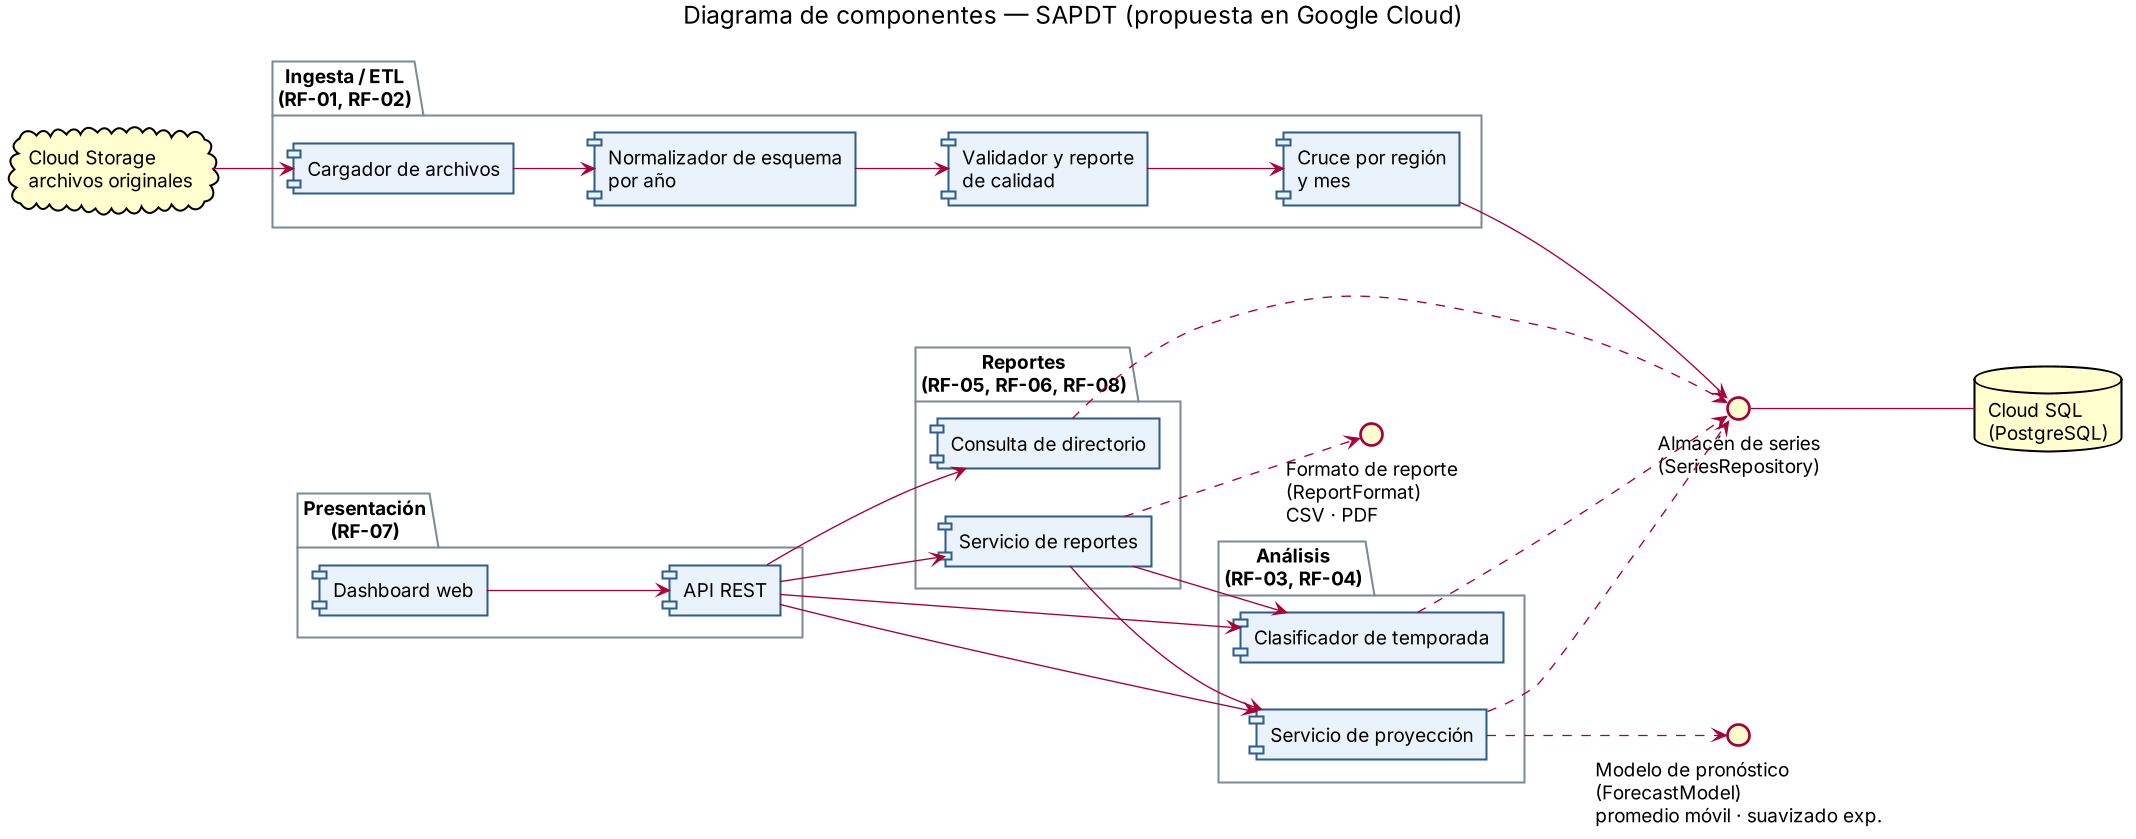
\includegraphics[width=\columnwidth]{CS_HITO1_componentes.png}
\caption{Diagrama de componentes propuesto en Google Cloud.}\label{fig:componentes}
\end{figure}

Ambos servicios se despliegan como contenedores en Google Cloud Run (proyecto \texttt{sapdt-lasalle}, región \texttt{us-central1}): \texttt{sapdt-api} y \texttt{sapdt-web} \cite{cloudrun}. Cloud Run escala a cero cuando no hay tráfico, por lo que el costo esperado para el curso es prácticamente nulo. El diseño inicial contemplaba Cloud SQL (PostgreSQL); se reemplazó por SQLite empaquetada en el contenedor porque los datos son de solo lectura, lo que evita el costo mensual de la base y la migración. Esta desviación debe revisarse si el sistema pasa a recibir datos nuevos a diario. La API solo acepta llamadas desde el origen de la interfaz, configurado por variable de entorno.

\section{Resultados y pruebas}\label{sec:resultados}
\subsection{Calidad de la carga y del cruce}
La Tabla~\ref{tab:carga} resume la carga sobre los archivos reales. Ninguna fila fue rechazada y 243 se cargaron marcadas como observadas: 228 por valores raros (por ejemplo, tasas de ocupación fuera de 0--100\,\% o camas y habitaciones vacías) y 15 por reparación verificable, de las cuales 12 con dos correos separados por punto y coma, 2 con la dirección cortada y 1 con la dirección web mal escrita. Recargar los mismos archivos no duplica filas. El cruce produjo una serie de 25 regiones por 126 meses (3\,150 filas), sin huecos, sin regiones huérfanas y sin nombres distintos para un mismo código.

\begin{table}[t]
\caption{Resultado de la carga (RF-01)}\label{tab:carga}
\centering
\begin{tabular}{@{}lrrr@{}}
\toprule
Fuente & Leídas & Rechazadas & Observadas \\
\midrule
Ocupabilidad 2015--2025 & 61\,890 & 0 & 64 \\
Directorio de hospedajes & 5\,091 & 0 & 179 \\
\midrule
Total & 66\,981 & 0 & 243 \\
\bottomrule
\end{tabular}
\end{table}

\subsection{Proyección y temporadas}
Cada modelo se evaluó reservando los últimos 12 meses como validación en las 25 regiones (Tabla~\ref{tab:modelos}). El estacional ingenuo fue el mejor en 17 regiones, lo que coincide con lo reportado en la literatura sobre la competitividad de los métodos simples \cite{song2008}. La interfaz ofrece promedio móvil y suavizado exponencial, que son los pedidos por el requisito, y muestra el error junto a cada pronóstico; el estacional ingenuo se conserva como referencia en los reportes. La temporada se clasifica por percentiles de cada región (alta desde P75 y baja hasta P25), y 2020--2021 se marca como periodo atípico por la pandemia.

\begin{table}[t]
\caption{Error de los modelos de proyección (validación de 12 meses)}\label{tab:modelos}
\centering
\begin{tabular}{@{}lcc@{}}
\toprule
Modelo & MAPE medio & Mejor en \\
\midrule
Estacional ingenuo & 10,7\,\% & 17 de 25 \\
Suavizado exponencial & 11,8\,\% & 5 de 25 \\
Promedio móvil & 12,7\,\% & 3 de 25 \\
\bottomrule
\end{tabular}
\end{table}

El comparativo entre regiones muestra, por ejemplo, que entre 2023 y 2024 los arribos crecieron 36,9\,\% en Cusco, 21,5\,\% en Arequipa y 5,8\,\% en Lima. La Fig.~\ref{fig:proyecciones} muestra el simulador de proyecciones desplegado.

\begin{figure}[t]
\centering
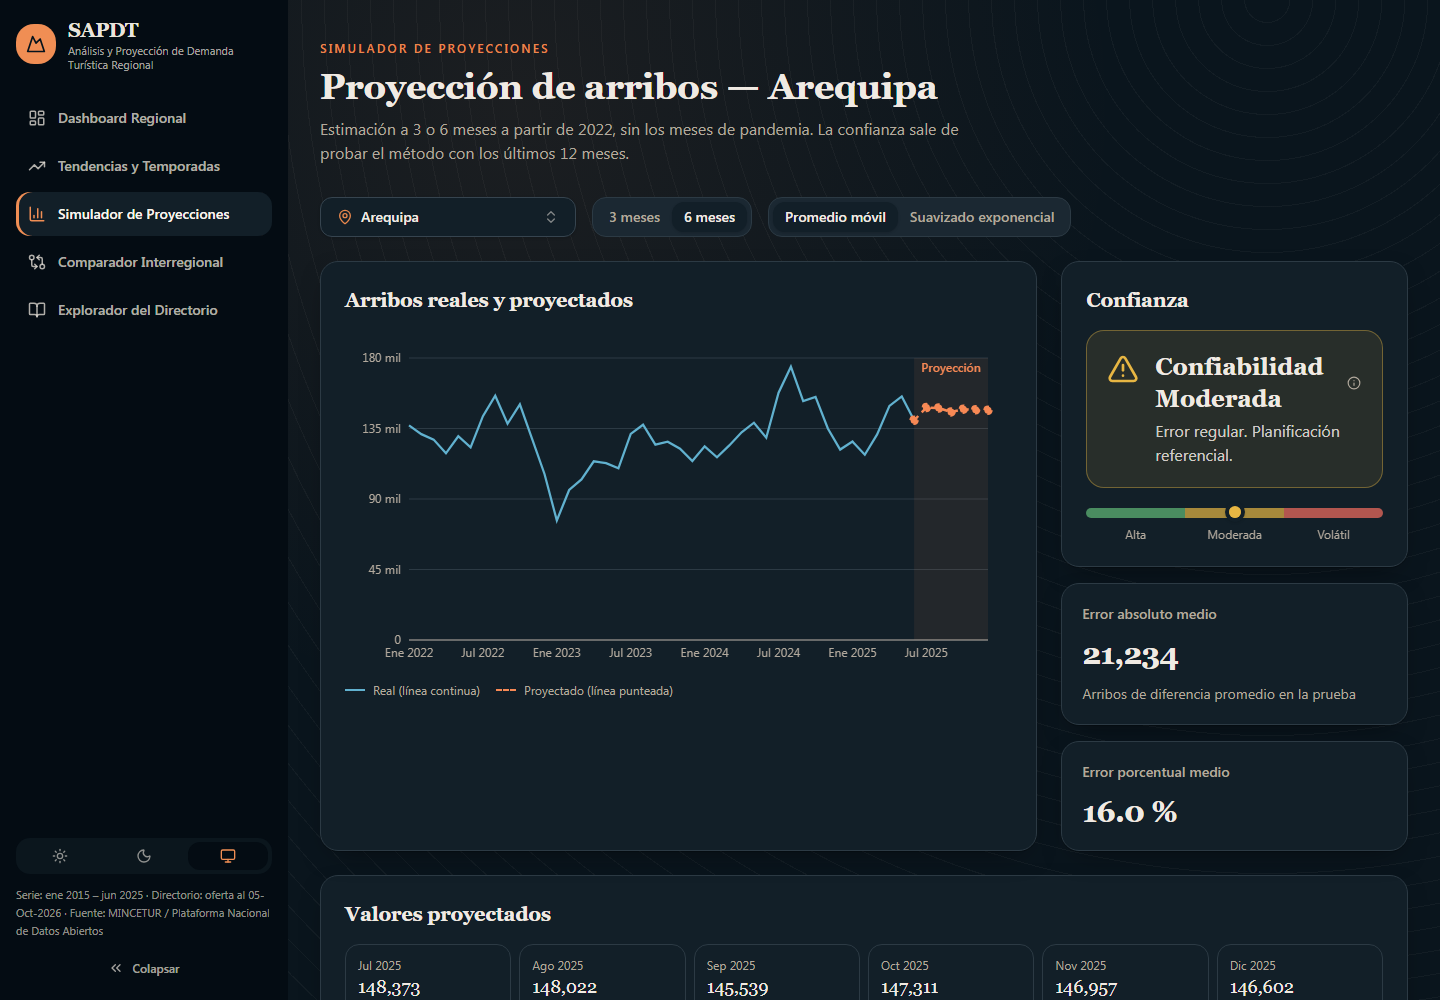
\includegraphics[width=\columnwidth]{proyecciones.png}
\caption{Simulador de proyecciones con nivel de confianza.}\label{fig:proyecciones}
\end{figure}

\subsection{Pruebas y verificación de los requisitos no funcionales}
La Tabla~\ref{tab:pruebas} relaciona cada nivel de prueba con su técnica y su evidencia en el repositorio. Las pruebas de Python se ejecutan sin framework con \texttt{python -m tests.<módulo>} y las de la interfaz con Vitest; todas pasan sobre la versión entregada. La Tabla~\ref{tab:evidencia} resume la evidencia de cada requisito no funcional.

\begin{table}[t]
\caption{Niveles y técnicas de prueba aplicados}\label{tab:pruebas}
\centering
\begin{tabular}{@{}p{1.6cm}p{2.4cm}p{3.6cm}@{}}
\toprule
Nivel & Técnica & Evidencia \\
\midrule
Componente & Partición de equivalencia & Ingesta: fila válida con coma decimal se carga, fila no numérica se rechaza; archivo de esquema desconocido se rechaza completo \\
Componente & Valores límite & Región con menos de 24 meses marcada ``no confiable''; reparación solo si quedan 28 campos verificables \\
Componente & Casos de uso / reglas & Cruce: solo filas consolidadas; huérfanos listados en ambos sentidos \\
Integración & Caja negra y pruebas negativas & API: rangos fuera de datos (400), región inexistente (404), formato no soportado (400); CSV y PDF válidos \\
Componente (web) & Valores límite y oráculo externo & 13 pruebas Vitest: percentiles, variación con base cero, totales nacionales 2019 y 2024 \\
Sistema & Verificación manual & Cinco pantallas con datos reales en Cloud Run \\
Regresión & Re-ejecución & Toda la batería tras cada cambio \\
\bottomrule
\end{tabular}
\end{table}

\begin{table}[t]
\caption{Evidencia de los requisitos no funcionales}\label{tab:evidencia}
\centering
\begin{tabular}{@{}lp{4.6cm}l@{}}
\toprule
ID & Evidencia & Estado \\
\midrule
RNF-01 & 243 filas observadas (15 reparadas), todas en el reporte & Cumple \\
RNF-02 & Código final: modelo nuevo en reportes, 0 clases; en la API, 2 funciones y la interfaz; formato nuevo, 1 función & Parcial \\
RNF-03 & Pruebas con bases pequeñas de ejemplo & Cumple \\
RNF-04 & Carga todo o nada; recargar no duplica & Cumple \\
RNF-05 & Serie completa en Cloud Run: mediana 0,44\,s, máximo 0,48\,s & Cumple \\
RNF-06 & Despliegue en Cloud Run con variables de entorno & Cumple \\
\bottomrule
\end{tabular}
\end{table}

\subsection{Métricas de calidad del código}
Se midieron dos métricas propuestas en el curso (Tabla~\ref{tab:metricas}). En el paquete \texttt{sapdt} del backend se midieron la cobertura de sentencias y de ramas con \texttt{coverage.py} al ejecutar las cuatro baterías de pruebas, y la complejidad ciclomática de McCabe \cite{mccabe1976} con \texttt{radon}. Se excluyeron de la cobertura los dos scripts de línea de comandos (\texttt{cargar.py} y \texttt{reportes.py}), que se ejecutan a mano y no tienen pruebas. Las funciones de mayor complejidad son la carga de un archivo (\texttt{IngestService.cargar}, 30) y la generación del reporte de calidad (21); son las candidatas a dividir en una siguiente iteración. En la interfaz web, la cobertura de Vitest es baja (27,2\,\% de sentencias) porque las 13 pruebas se concentran en el módulo de dominio (52,0\,\%) y no cubren los componentes visuales.

\subsection{Modificabilidad y eficiencia en la nube}
Para RNF-02 se repitió sobre el código final la prueba hecha en la Práctica 2: se agregó un modelo de proyección nuevo (media histórica) en una copia del código. En el módulo de análisis que genera los reportes bastó una clase nueva y su registro en el diccionario de modelos, sin modificar ninguna clase existente, y las pruebas siguieron pasando. En cambio, la API que usa la interfaz implementa sus dos modelos con condicionales, por lo que ofrecer el modelo nuevo en pantalla exige cambiar dos funciones de la API y el selector de la interfaz; agregar un formato de exportación toca una sola función. Por eso RNF-02 se cumple solo en parte, y unificar la API con el registro de modelos queda como mejora.

Para RNF-05 se midió el tiempo de respuesta de la API desplegada desde un navegador en el Perú el 23 de noviembre de 2026, con 15 solicitudes por servicio y la instancia ya activa. La serie regional completa respondió con una mediana de 0,44\,s (máximo 0,48\,s); temporada, proyección, comparativo y directorio, con medianas entre 0,23 y 0,25\,s; y la exportación del directorio a PDF, con 0,83\,s. Todos quedan por debajo del límite de 2\,s. No se midió el arranque en frío de Cloud Run.

[POR COMPLETAR: la eficiencia de detección de defectos (DDE) y las pruebas de aceptación con usuarios aún no se miden; agregarlas aquí si el equipo las obtiene.]

\begin{table}[t]
\caption{Métricas de calidad del código}\label{tab:metricas}
\centering
\begin{tabular}{@{}lr@{}}
\toprule
Métrica & Valor \\
\midrule
Cobertura de sentencias & 81,6\,\% (529 de 648) \\
Cobertura de ramas & 69,9\,\% (144 de 206) \\
Cobertura web, sentencias (todo / dominio) & 27,2\,\% / 52,0\,\% \\
Funciones y métodos analizados & 69 \\
Complejidad ciclomática media & 5,8 \\
Funciones con complejidad $\leq 10$ & 55 (80\,\%) \\
Complejidad máxima & 30 \\
\bottomrule
\end{tabular}
\end{table}


\section{Relación con la ISO/IEC 42001}\label{sec:42001}
SAPDT no está certificado en la ISO/IEC 42001 ni implementa un sistema de gestión de IA: es un proyecto de curso y sus modelos de proyección son métodos estadísticos simples, no aprendizaje automático. Sin embargo, el enunciado del curso invita a incorporar aprendizaje automático, y si una versión futura lo hiciera, la norma daría un marco para gobernarlo. Varias prácticas del proyecto ya apuntan en la dirección de sus controles. Para los datos (A.7), el origen de cada archivo, su preparación y sus problemas de calidad quedan registrados en el reporte de cada carga. Para el ciclo de vida (A.6), cada modelo se valida con un tramo de 12 meses reservados y su error se publica junto al pronóstico. Para la evaluación de impactos (A.5), la regla de ``no confiable'' con menos de 24 meses y el aviso de periodo atípico limitan el uso indebido de un pronóstico. Lo que faltaría es lo propio de un sistema de gestión: una política de IA, roles y responsabilidades, una evaluación formal de riesgos e impactos, y auditorías y revisiones periódicas.

\section{Conclusiones}\label{sec:conclusiones}
SAPDT cumple los ocho requisitos funcionales sobre datos abiertos reales y está desplegado en Google Cloud Run. El enfoque de calidad del proyecto se reflejó en que la carga no perdió ninguna de las 66\,981 filas en silencio: cada observación y cada reparación quedó registrada y probada. La evaluación de los modelos de proyección mostró errores medios de 10,7\,\% a 12,7\,\%, por lo que el sistema muestra siempre el error junto al pronóstico en lugar de presentarlo como una cifra exacta.

Las principales limitaciones son que los datos llegan solo hasta junio de 2025, que el PDF exportado es una tabla sencilla y que la API no aprovecha aún el registro de modelos intercambiables del módulo de análisis. Como trabajo futuro se propone documentar las pruebas según IEEE 829, subir la cobertura de ramas y dividir las funciones de complejidad mayor a 10, incorporar modelos estacionales con tendencia, automatizar la descarga periódica desde el portal y, si los datos pasan a actualizarse con frecuencia, migrar la base a un servicio administrado. El código, la documentación y la guía de despliegue están en \url{https://github.com/leonardouwz/sapdt}, y la aplicación en \url{https://sapdt-web-606560700752.us-central1.run.app}.

\begin{thebibliography}{99}
\bibitem{pnda} Plataforma Nacional de Datos Abiertos, ``Indicadores de ocupabilidad de los establecimientos de hospedaje y Directorio de establecimientos de hospedaje calificados,'' MINCETUR, 2025. [En línea]. Disponible: \url{https://www.datosabiertos.gob.pe}
\bibitem{mincetur} Ministerio de Comercio Exterior y Turismo, ``Estadísticas de turismo,'' MINCETUR, Lima, Perú. [En línea]. Disponible: \url{https://www.gob.pe/mincetur}
\bibitem{song2008} H. Song y G. Li, ``Tourism demand modelling and forecasting---A review of recent research,'' \emph{Tourism Management}, vol. 29, no. 2, pp. 203--220, 2008.
\bibitem{hyndman2021} R. J. Hyndman y G. Athanasopoulos, \emph{Forecasting: Principles and Practice}, 3rd ed. Melbourne, Australia: OTexts, 2021.
\bibitem{gardner1985} E. S. Gardner Jr., ``Exponential smoothing: The state of the art,'' \emph{Journal of Forecasting}, vol. 4, no. 1, pp. 1--28, 1985.
\bibitem{hyndman2006} R. J. Hyndman y A. B. Koehler, ``Another look at measures of forecast accuracy,'' \emph{International Journal of Forecasting}, vol. 22, no. 4, pp. 679--688, 2006.
\bibitem{wang1996} R. Y. Wang y D. M. Strong, ``Beyond accuracy: What data quality means to data consumers,'' \emph{Journal of Management Information Systems}, vol. 12, no. 4, pp. 5--33, 1996.
\bibitem{iso25012} ISO/IEC, \emph{Software engineering---Software product Quality Requirements and Evaluation (SQuaRE)---Data quality model}, ISO/IEC 25012:2008, 2008.
\bibitem{iso25010} ISO/IEC, \emph{Systems and software engineering---Systems and software Quality Requirements and Evaluation (SQuaRE)---System and software quality models}, ISO/IEC 25010:2011, 2011.
\bibitem{iso12207} ISO/IEC/IEEE, \emph{Systems and software engineering---Software life cycle processes}, ISO/IEC/IEEE 12207:2017, 2017.
\bibitem{ieee730} IEEE, \emph{IEEE Standard for Software Quality Assurance Plans}, IEEE Std 730-2002, 2002.
\bibitem{ieee829} IEEE, \emph{IEEE Standard for Software and System Test Documentation}, IEEE Std 829-2008, 2008.
\bibitem{istqb2023} International Software Testing Qualifications Board, \emph{Certified Tester Foundation Level Syllabus}, v4.0, 2023. [En línea]. Disponible: \url{https://www.istqb.org}
\bibitem{iso42001} ISO/IEC, \emph{Information technology---Artificial intelligence---Management system}, ISO/IEC 42001:2023, 1st ed., dic. 2023.
\bibitem{modulos42001} Modulos, ``ISO/IEC 42001:2023 Annexes A--D: Reference controls, implementation guidance, objectives, and sectors,'' Modulos Docs. [En línea]. Disponible: \url{https://docs.modulos.ai/frameworks/iso-42001/annexes-a-d.html}
\bibitem{scrum2020} K. Schwaber y J. Sutherland, \emph{The Scrum Guide}, 2020. [En línea]. Disponible: \url{https://scrumguides.org}
\bibitem{sommerville2011} I. Sommerville, \emph{Software Engineering}, 10th ed. Boston, MA, USA: Pearson, 2016.
\bibitem{ieee830} IEEE Computer Society, \emph{IEEE Recommended Practice for Software Requirements Specifications}, IEEE Std 830-1998, 1998.
\bibitem{pressman2020} R. S. Pressman y B. R. Maxim, \emph{Ingeniería del software: un enfoque práctico}, 9.ª ed. México: McGraw-Hill, 2020.
\bibitem{cloudrun} Google Cloud, ``Cloud Run documentation.'' [En línea]. Disponible: \url{https://cloud.google.com/run/docs}
\bibitem{mccabe1976} T. J. McCabe, ``A complexity measure,'' \emph{IEEE Transactions on Software Engineering}, vol. SE-2, no. 4, pp. 308--320, 1976.
\end{thebibliography}

\end{document}
